\chapter{Circuits' topology optimization focused on the performance improvement and functionalities integration as a way of power loss reduction}\label{performance}

\indent In this Chapter the approach of circuits' topology optimization focused on the performance improvement and functionality integration as a way of power loss minimization is presented. More effective circuits' topologies of directional filters and directional couplers were studied allowing to obtain a given required electrical performance while reducing the overall circuits size and/or complexity which as a result leads to the reduction of total length of the wave's propagation path, therefore reduced power loss.
\\
\indent Modern communication systems require an integration of many frequency bands with preferably a single aperture to cover the desired frequencies (e.g., GPS, GSM, WLAN and UWB bands). For such front-end systems, there is a need for broadband antennas on one hand, and devices for multiplexing signals in the frequency domain on the other hand. Devices constructed of directional filters (DFs) can perform multiplexing function \cite{mm_cameron}, while featuring the advantage of low reflection at the input over wide bandwidth and modular topology, in which filters for each band can be designed separately. Furthermore, such devices can easily be integrated with passive and active circuits, effectively increasing system’s integration and lowering the total power loss. Channel selectivity of a multiplexer is dependent from the realization of constitutive DFs, thus highly selective directional filters are of need.
\\
\indent Following the signal path within a wireless transceiver front-end, a power amplification stage is of interest. For low-noise low-power amplifiers MMIC circuits are usually used, whereas for high-power amplifiers, a power transistor based solutions are utilized. Apart from active components, passive power division/summation and/or impedance matching networks are needed, which are rather bulky components. Therefore, a compact and low-loss networks are of importance, hence the integration of power division and impedance transformation functionality \cite{tmtt_wincza_asymmetric_transformers} would be advantageous. Moreover, to allow for realization of broadband amplification stage covering more than one frequency band of interest, broadband directional couplers are required as they are basic components for multi-channel or balanced amplifiers.
\\
\indent The Author has proposed and developed various novel circuits and design methodologies of highly-selective directional filters and frequency multiplexers as well as impedance transforming or broadband directional couplers. Results of the conducted research have been a subject of three journal papers: one submitted to \textit{IEEE Transactions on Microwave Theory and Techniques}, two published in and one submitted to \textit{IEEE Microwave and Wireless Components Letters} and one published in \textit{International Journal of Microwave and Wireless Technologies} as well as two conference papers presented at \textit{International Symposium on Antennas and Propagation ISAP'15} and \textit{International Conference on Microwave, Radar and Wireless Communications MIKON'16}, both under the auspices of \textit{Institute of Electrical and Electronics Engineers IEEE}, which constitute the Chapter.
\\
\indent In Section \ref{pe:isap_df-min}, a new design of a miniaturized coupled-line directional-filters-based multiplexer allowing for band separation in UWB antenna systems has been proposed. To achieve small size of the directional filters, hence the entire multiplexer, directional couplers constituting the filter have been miniaturized following the   approach, in which the coupler is realized as a connection of tightly coupled and uncoupled lines. Moreover, sections of quarter-wave-long transmission lines have been designed with quasi-lumped elements approach, which allows for further miniaturization of the structure. Theoretical analysis of the circuit has been provided. Moreover, performance of the presented approach has been verified by the design and measurement of an exemplary single-channel directional filter multiplexer covering Industrial, Scientific and Medical (ISM) 2.4 GHz band.
\\
\indent Additionally, in Section \ref{pe:mwcl_df-dbrf}, a novel approach to the design of directional filters based on differential bandstop filters and delay lines is proposed. It is shown, that the utilization of a phase inverter and a reference line as a mode converting phase shifter allows for obtaining theoretically ideal bandpass to bandstop channels isolation over an infinite bandwidth. The presented theoretical analysis is confirmed by the realization of an exemplary low-loss directional filter with defected ground type phase inverter covering  ISM 2.4 GHz band. The obtained measurement results show insertion loss as low as 1.1 dB and almost flat isolation response, better than 27 dB up to 6 GHz proving the validity of the presented approach.
\\
\indent Moreover, in Section \ref{pe:tmtt_df-zeros}, a novel topology of a traveling-wave directional filter allowing for selectivity enhancement without increasing filter’s order is proposed. Additional loose cross coupling introduced between $\#(n-1)^{th}$ loop resonator and isolated port of the $n^{th}$-order directional filter allows for generating transmission zeros in the bandpass branch. Moreover, electrical length of the cross coupling connecting transmission line allows for adjusting the location of transmission zeros and realizing symmetric or asymmetric frequency response. The presented approach is theoretically analyzed and experimentally verified. Exemplary second- and third-order directional filters with symmetrically placed transmission zeros were designed to operate at the center frequency $f_0$ = 1 GHz, manufactured and measured. The obtained results prove the correctness and applicability of the presented approach.
\\
\indent Following, in Section \ref{pe:mikon_df-zeros}, a new design of a traveling wave loop directional filter allowing for the realization of transmission zeroes has been proposed. In order to introduce transmission zeroes to bandpass branch of the filter, two loops have been cascaded using transmission line sections. Theoretical analysis of the circuit has been provided giving the insight into behavior of the appearing transmission zeroes related to electrical lengths of the loops’ connecting section. Performance of the presented approach has been verified by the design and measurements of an exemplary cascaded single-loops directional filter with two symmetrically placed transmission zeroes covering ISM 2.4 GHz band. The obtained results proved the usefulness of the presented approach.
\\
\indent Further, in Section \ref{pe:mwcl_multiplexer}, a novel approach to the design of frequency multiplexers consisting of cascaded directional filters is proposed. It is shown that when channels are spaced closely enough, their selectivity can be improved without increasing filters' order by taking advantage of two phenomena. Asymmetric frequency response of a constitutive directional filter allows to increase the attenuation slope on one side of the multiplexer channel. Additionally, the slope on the other side can be increased due to the creation of additional transmission zero resulting from the fact that bandstop response of previous directional filters within the cascade affects directly the response of the following channel. Theoretical analysis is provided together with the applicability condition and multiplexer's design procedure. Moreover, an exemplary four-channel S-band multiplexer was manufactured and measured showing the selectivity improvement of as much as $\sim$ 1.3 times.
\\
\indent Finally, in Section \ref{pe:jmwt_imp-coupler}, a novel impedance transforming directional couplers are proposed in which the achievable impedance transformation ratio is increased above the previously reported limit related to coupling of the coupled-line sections. The proposed couplers consist of two coupled-line sections between which uncoupled sections of LH lines are connected. The presented concept has been verified by circuit simulations as well as by measurements of the manufactured 3-dB coupled-line impedance transforming directional coupler operating at the center frequency $f\textsubscript{0}$ = 1.2 GHz and featuring twofold increase of the impedance transformation ratio compared to a classic solution being $R$ = 4.
\\
\indent Besides, in Section \ref{pe:mwcl_tandem}, a new type of a broadband 3-dB tandem coupler has been proposed featuring frequency characteristics of the resulting coupling similar to these of a classic 3-dB two-section asymmetric coupled-line directional coupler. The coupler is composed of two loosely-coupled-line sections having electrical length close to quarter-wavelength connected by right-handed and left-handed transmission line sections. Theoretical analysis and design equations have been presented with exemplary realization. Measurements of the manufactured tandem coupler operating at the center frequency $f\textsubscript{0}$ = 1 GHz having wide operational bandwidth have been shown to validate the presented analysis.

\cleardoublepage

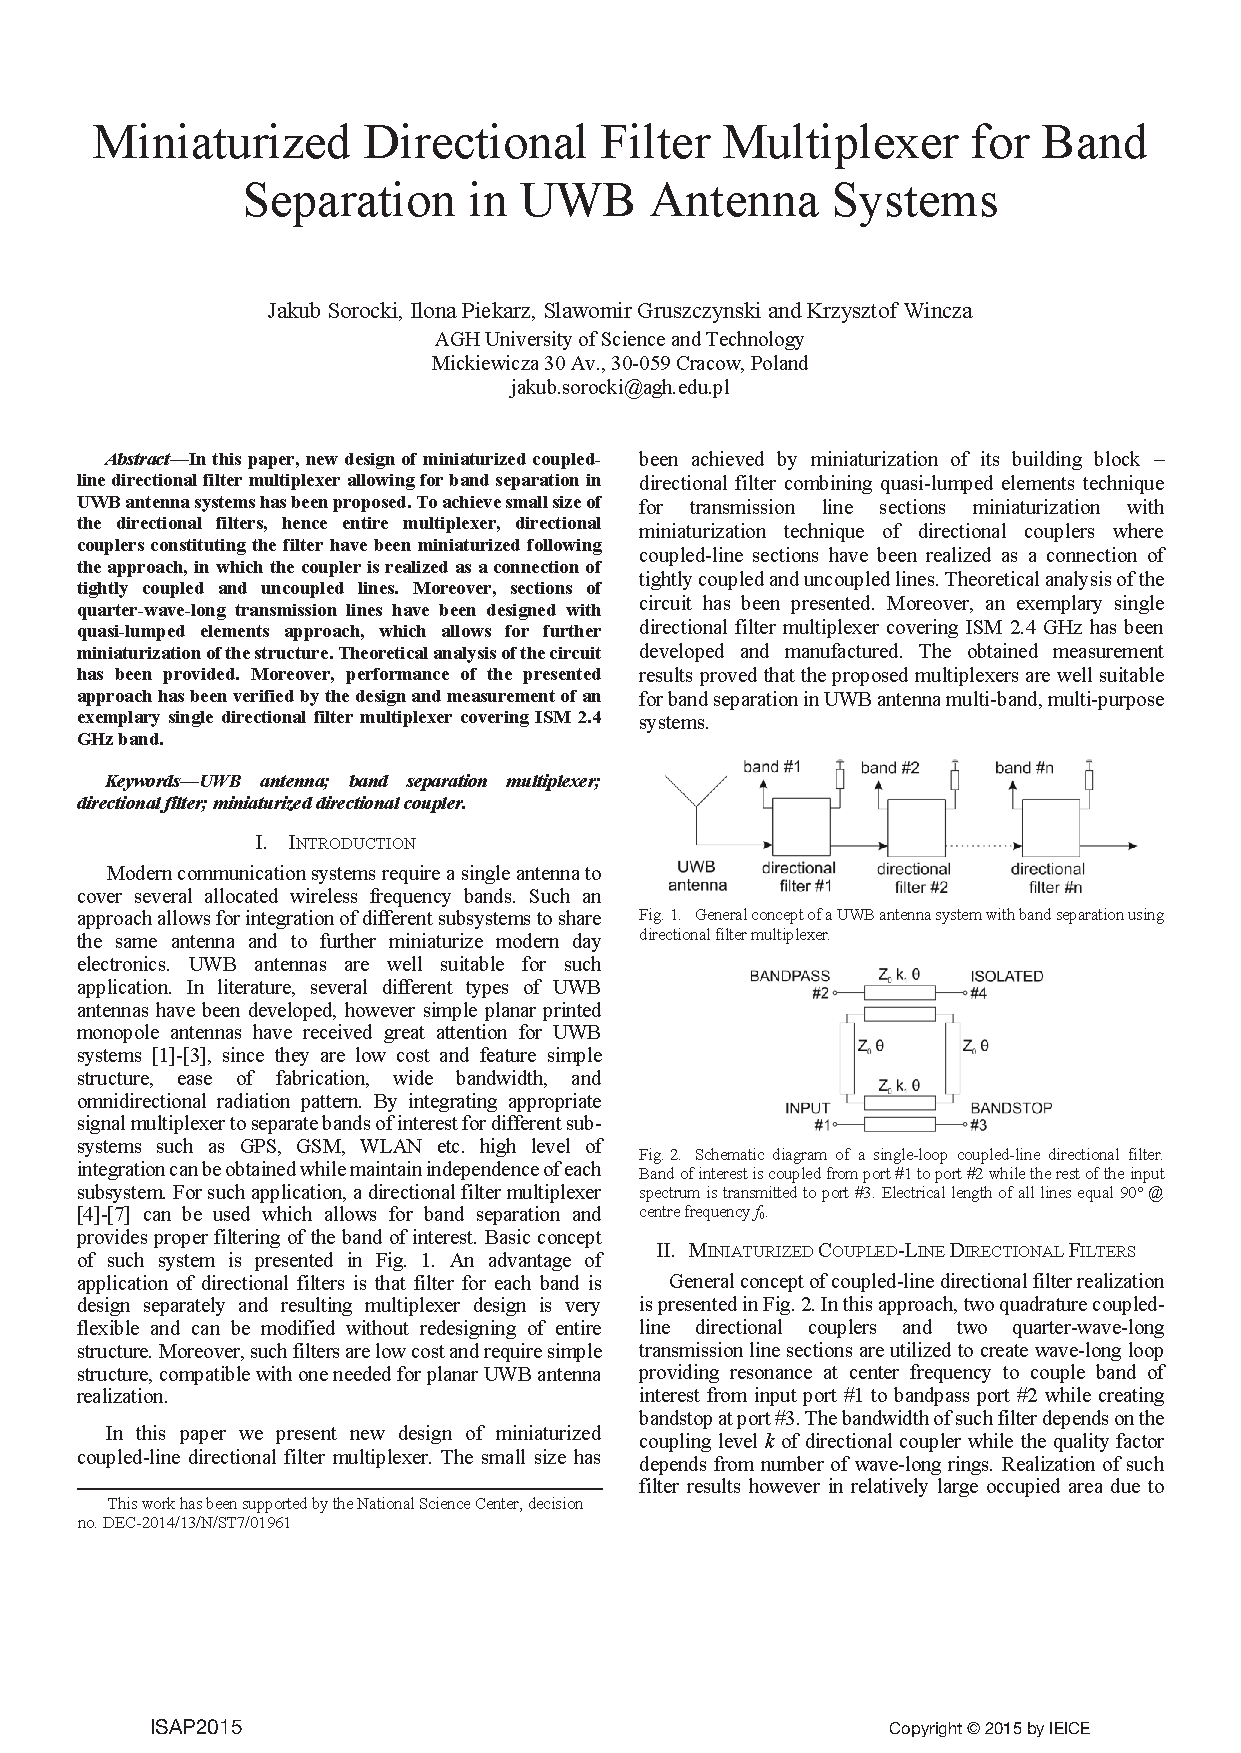
\includepdf[pages=-,addtotoc={1,section,1,Miniaturized directional filter multiplexer for band separation in UWB antenna systems,pe:isap_df-min}, pagecommand={}, scale=.97]{chapter_4/isap_df-min.pdf}

\cleardoublepage

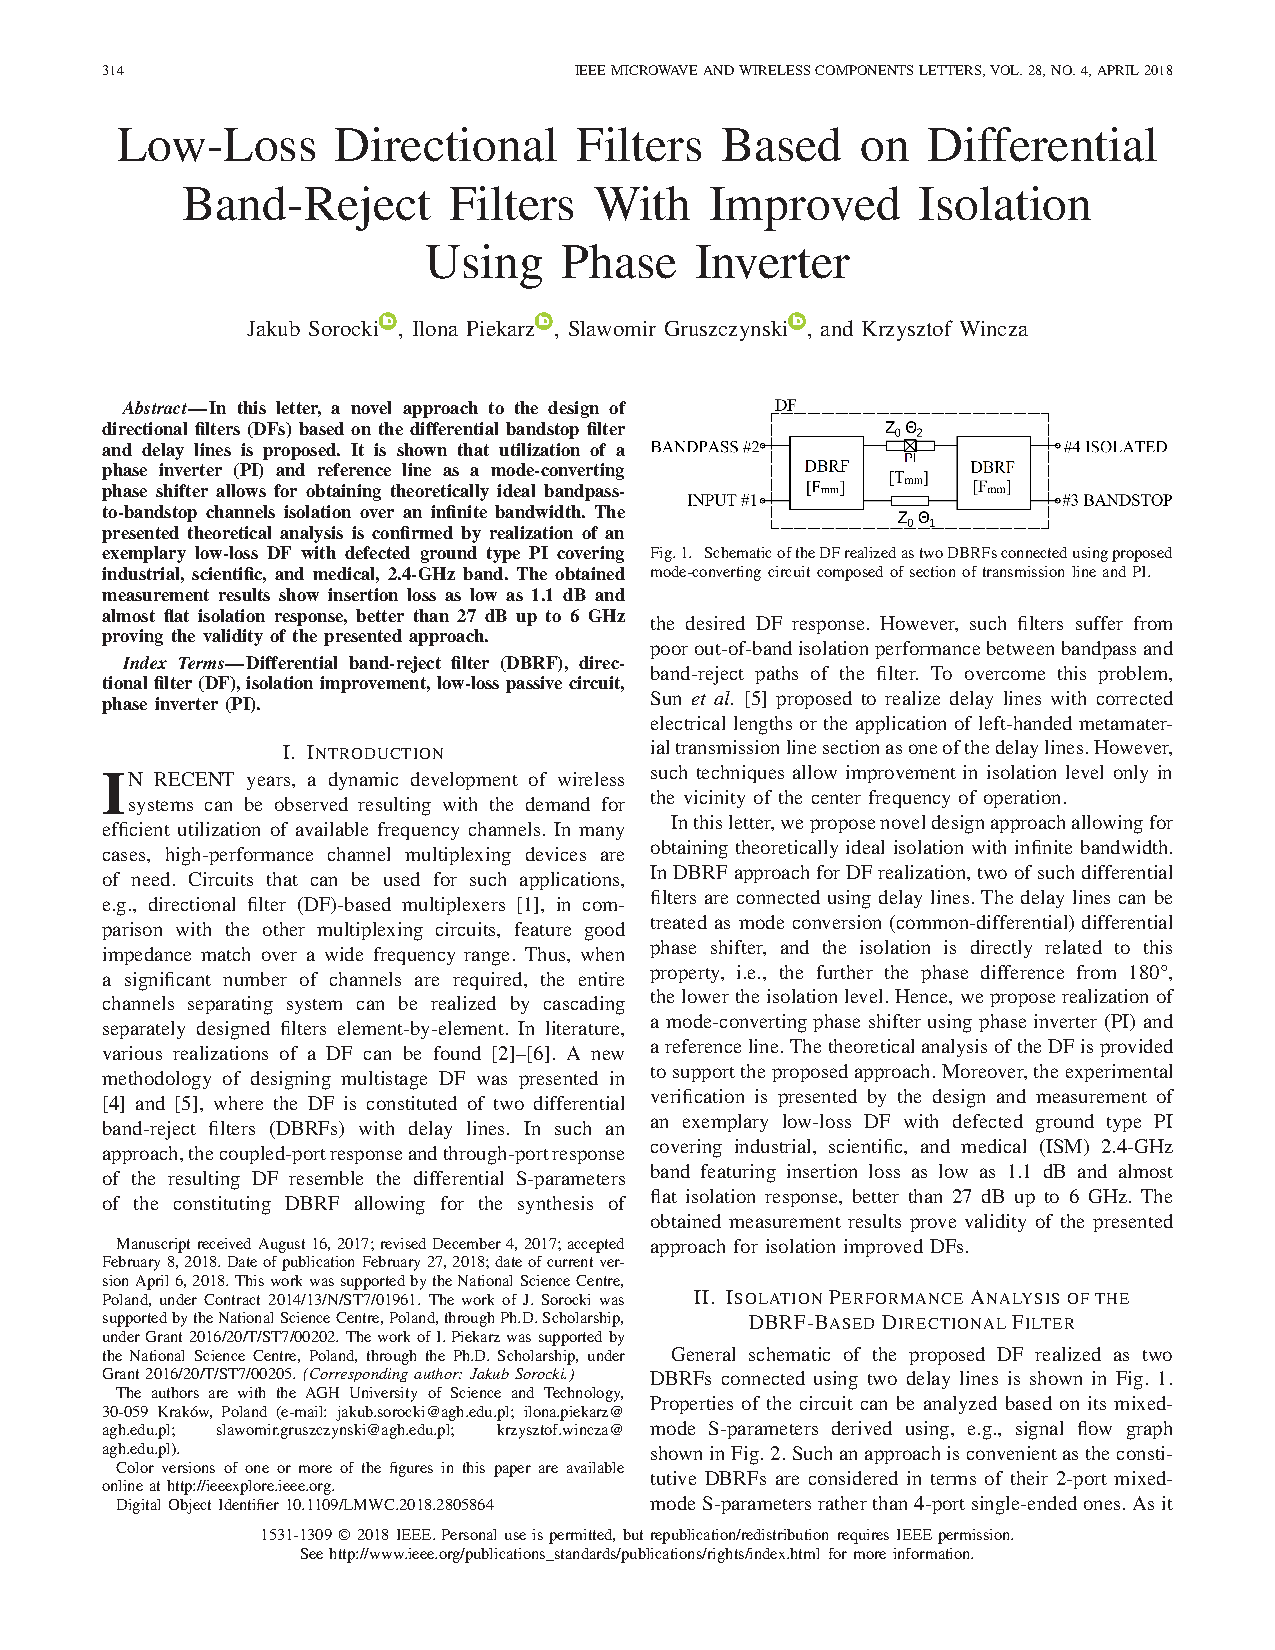
\includepdf[pages=-,addtotoc={1,section,1,Low-loss directional filters based on differential band-reject filters with improved isolation using phase inverter,pe:mwcl_df-dbrf}, pagecommand={}, scale=.97]{chapter_4/mwcl_df-dbrf.pdf}

\cleardoublepage

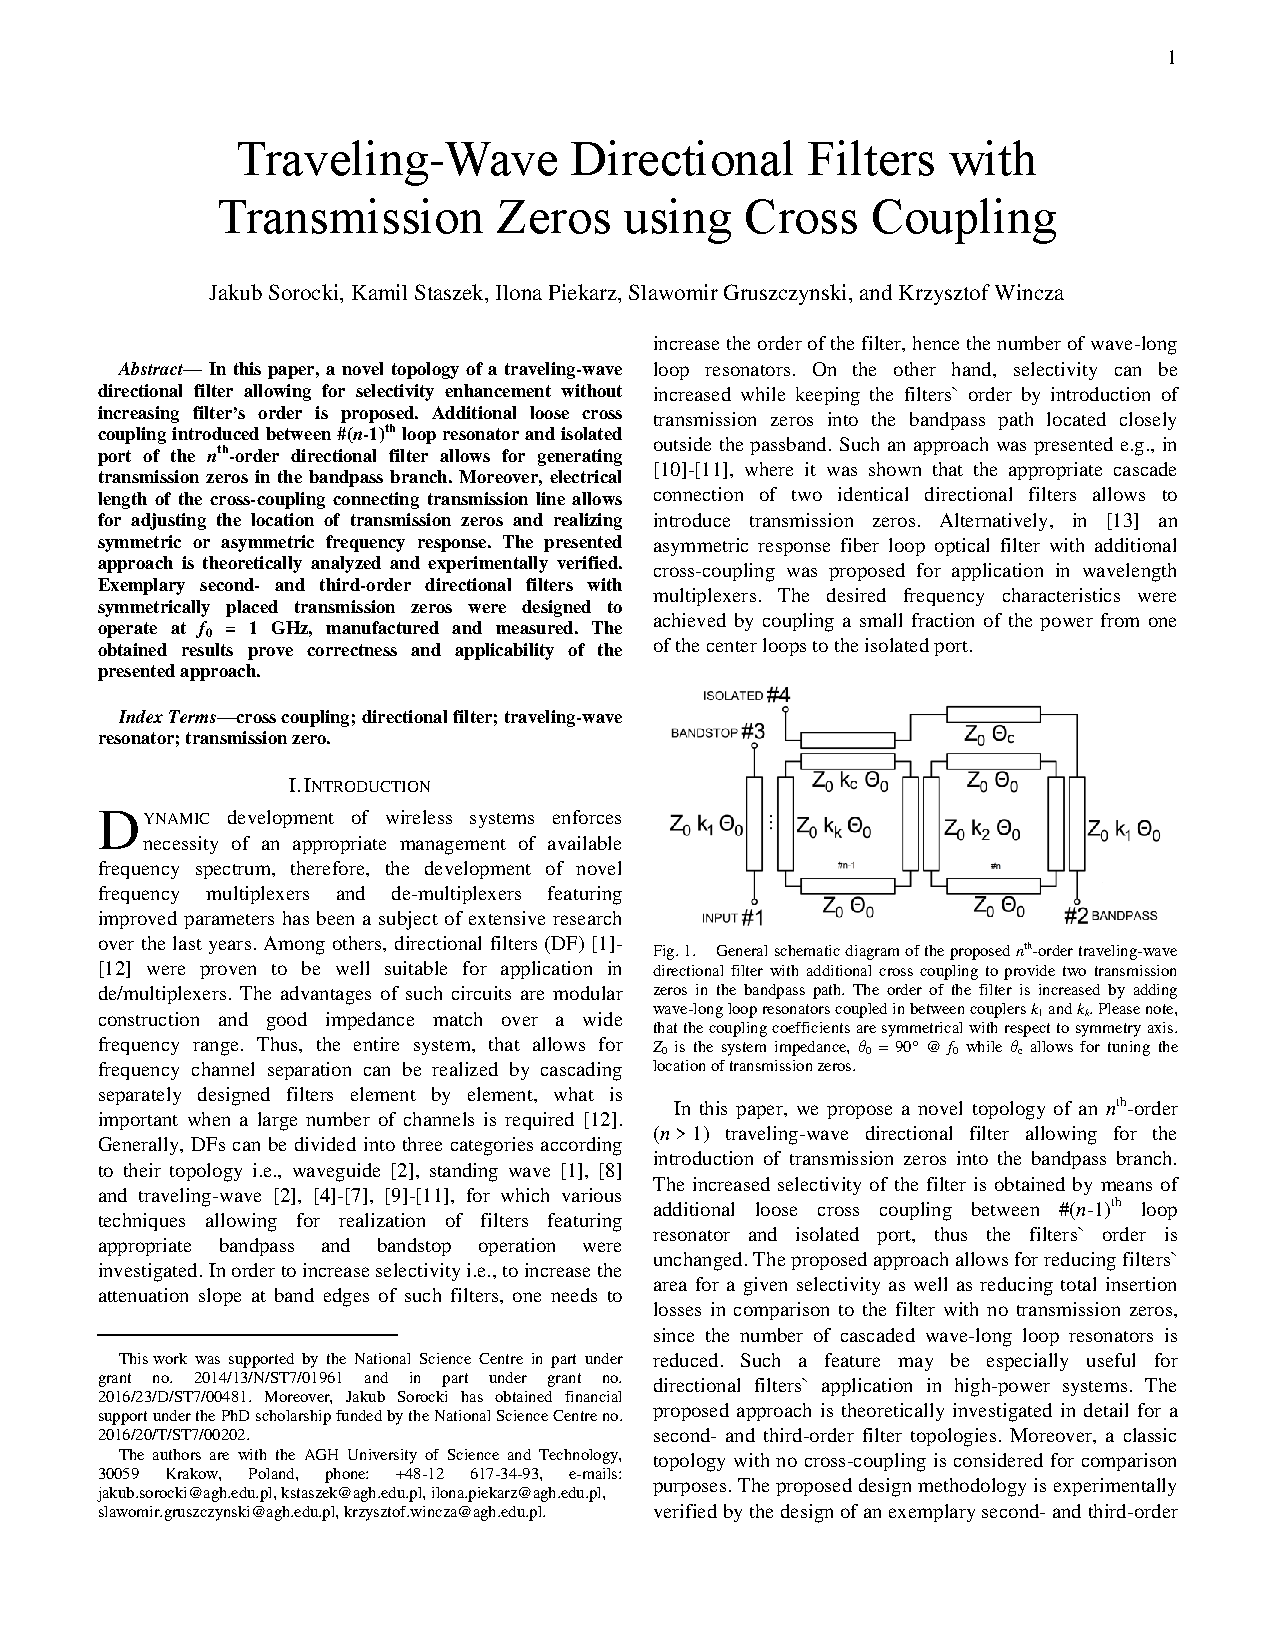
\includepdf[pages=-,addtotoc={1,section,1,Traveling wave directional filters with transmission zeroes using cross coupling,pe:tmtt_df-zeros}, pagecommand={}, scale=.97]{chapter_4/tmtt_df-zeros.pdf}

\cleardoublepage

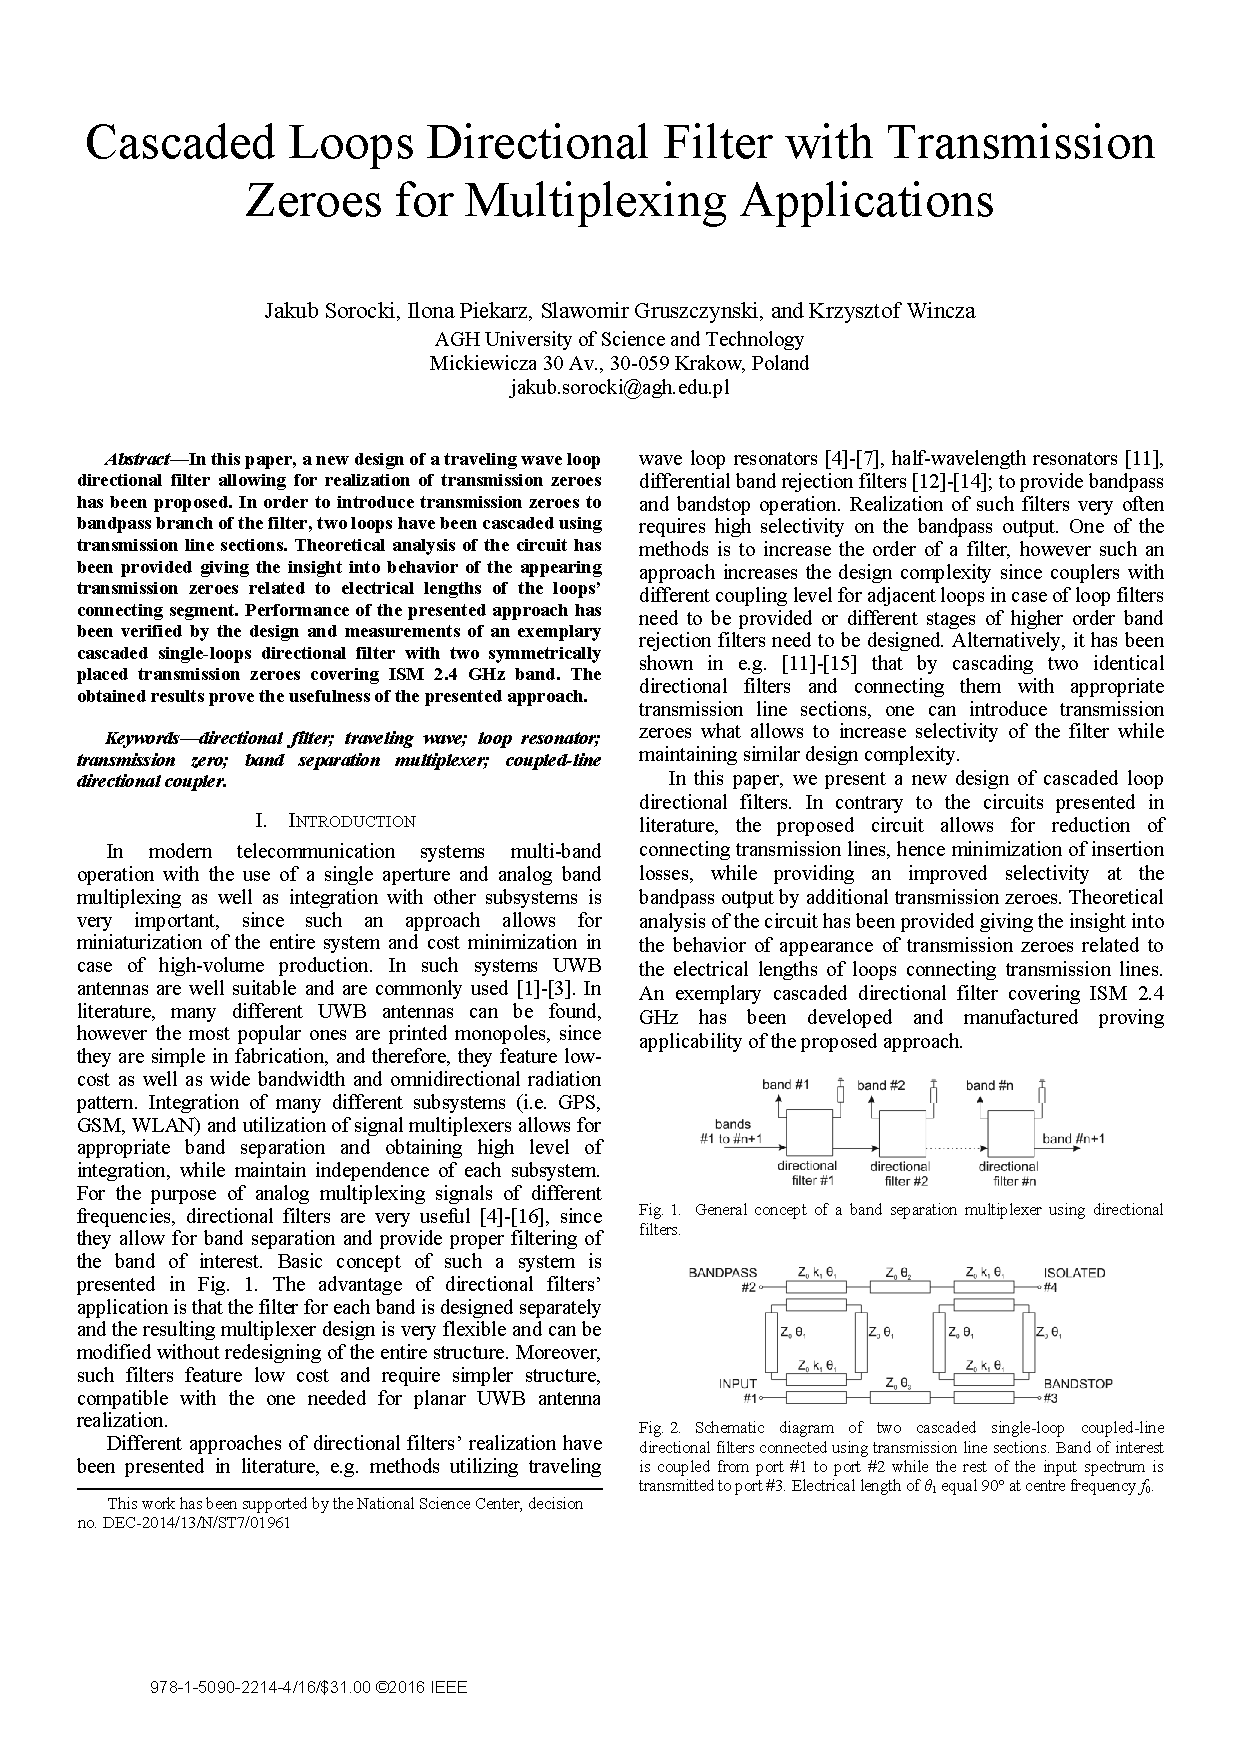
\includepdf[pages=-,addtotoc={1,section,1,Cascaded loops directional filter with transmission zeroes for multiplexing applications,pe:mikon_df-zeros}, pagecommand={}, scale=.97]{chapter_4/mikon_df-zeros.pdf}


\cleardoublepage

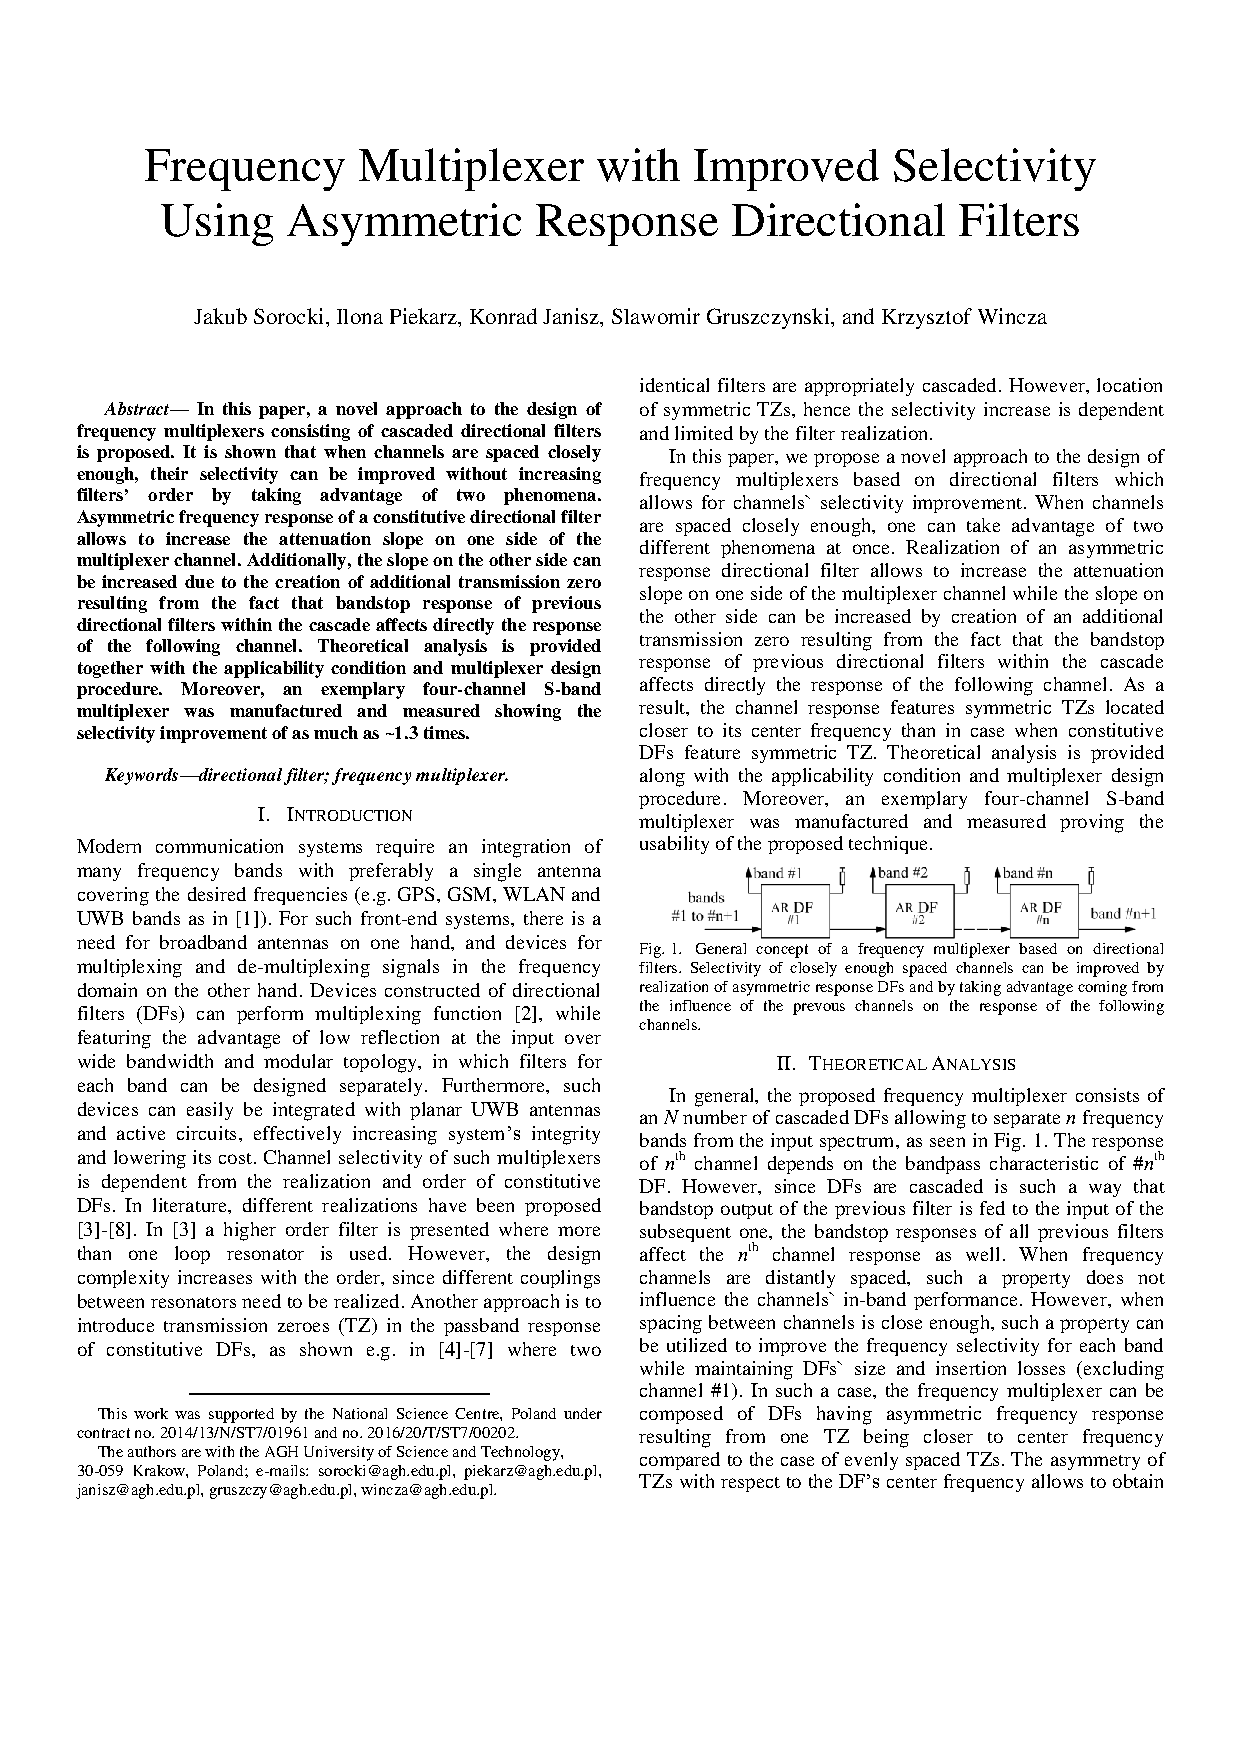
\includepdf[pages=-,addtotoc={1,section,1,Frequency multiplexers with improved selectivity using asymmetric response directional filters,pe:mwcl_multiplexer}, pagecommand={}, scale=.97]{chapter_4/mwcl_multiplexer.pdf}

\cleardoublepage

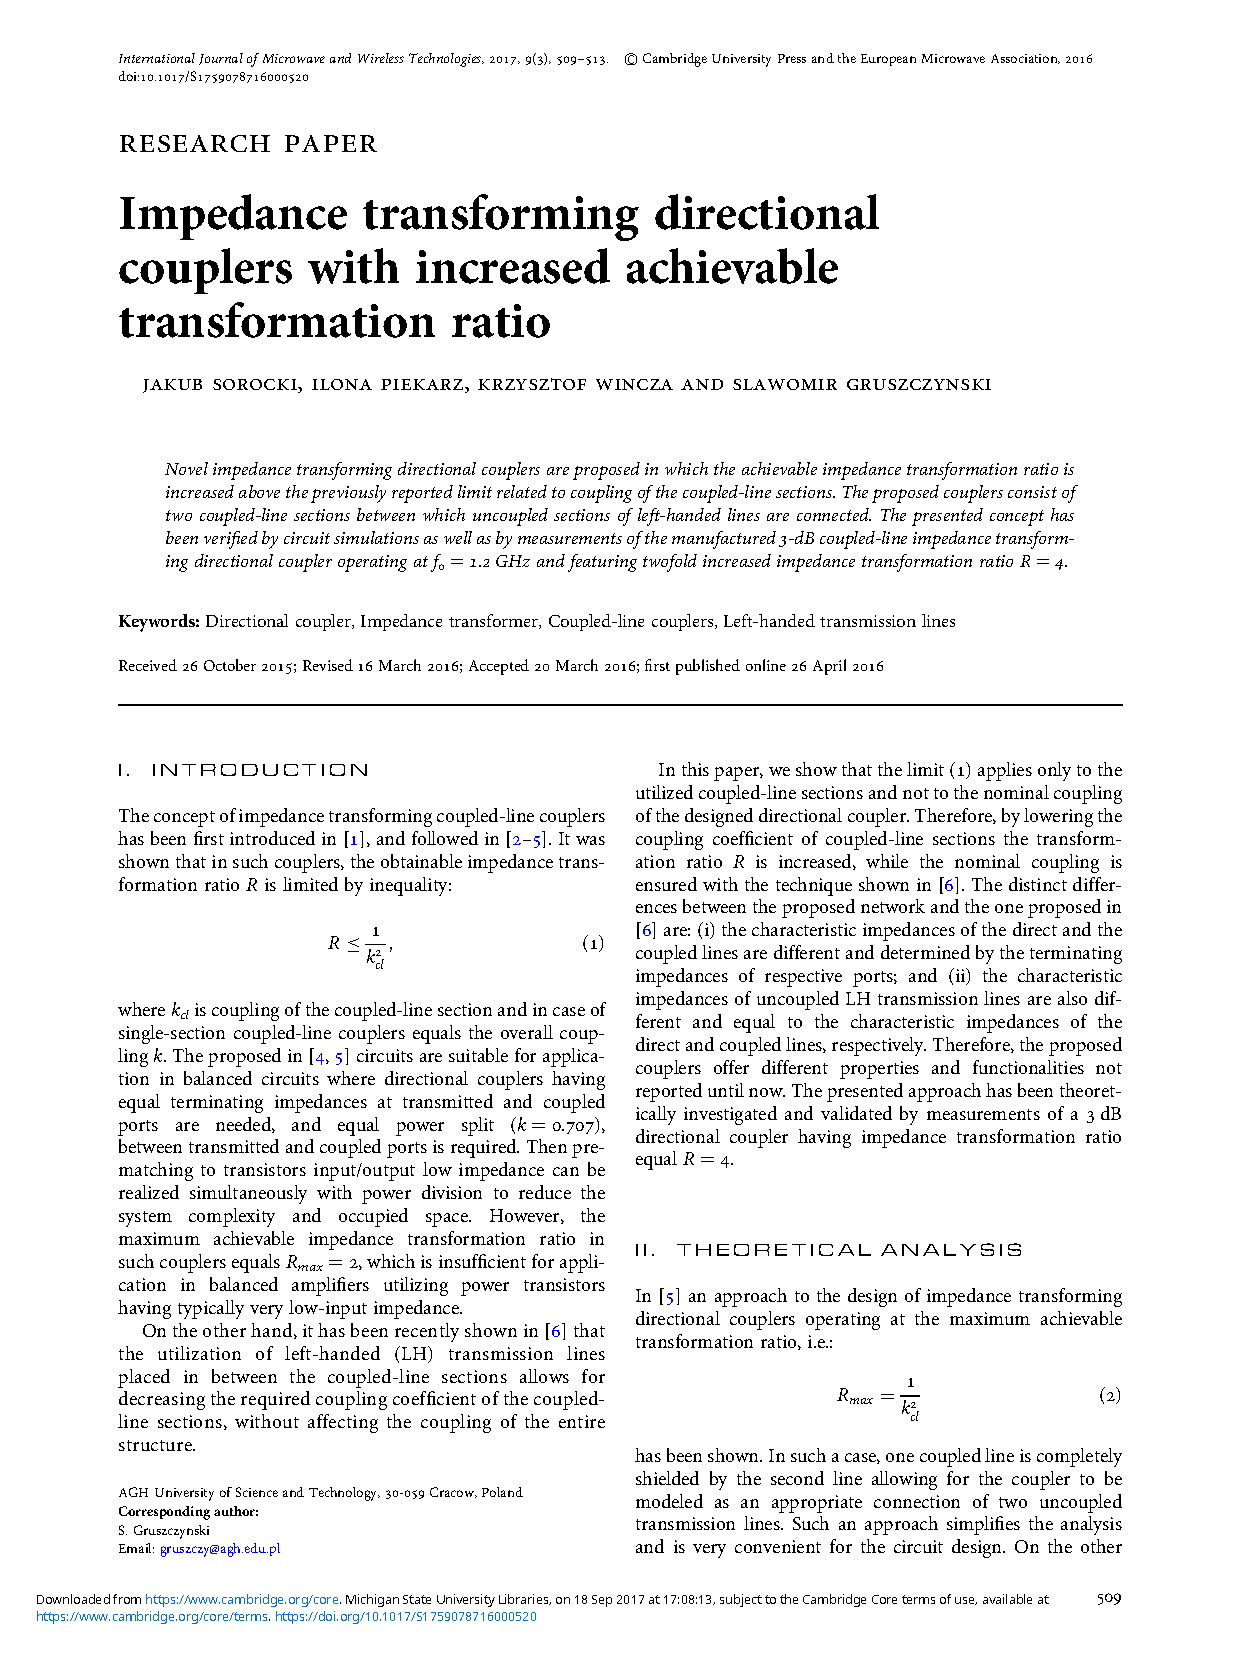
\includepdf[pages=-,addtotoc={1,section,1,Impedance transforming directional couplers  with increased achievable transformation ratio,pe:jmwt_imp-coupler}, pagecommand={}, scale=.97]{chapter_4/jmwt_imp-coupler.pdf}

\cleardoublepage

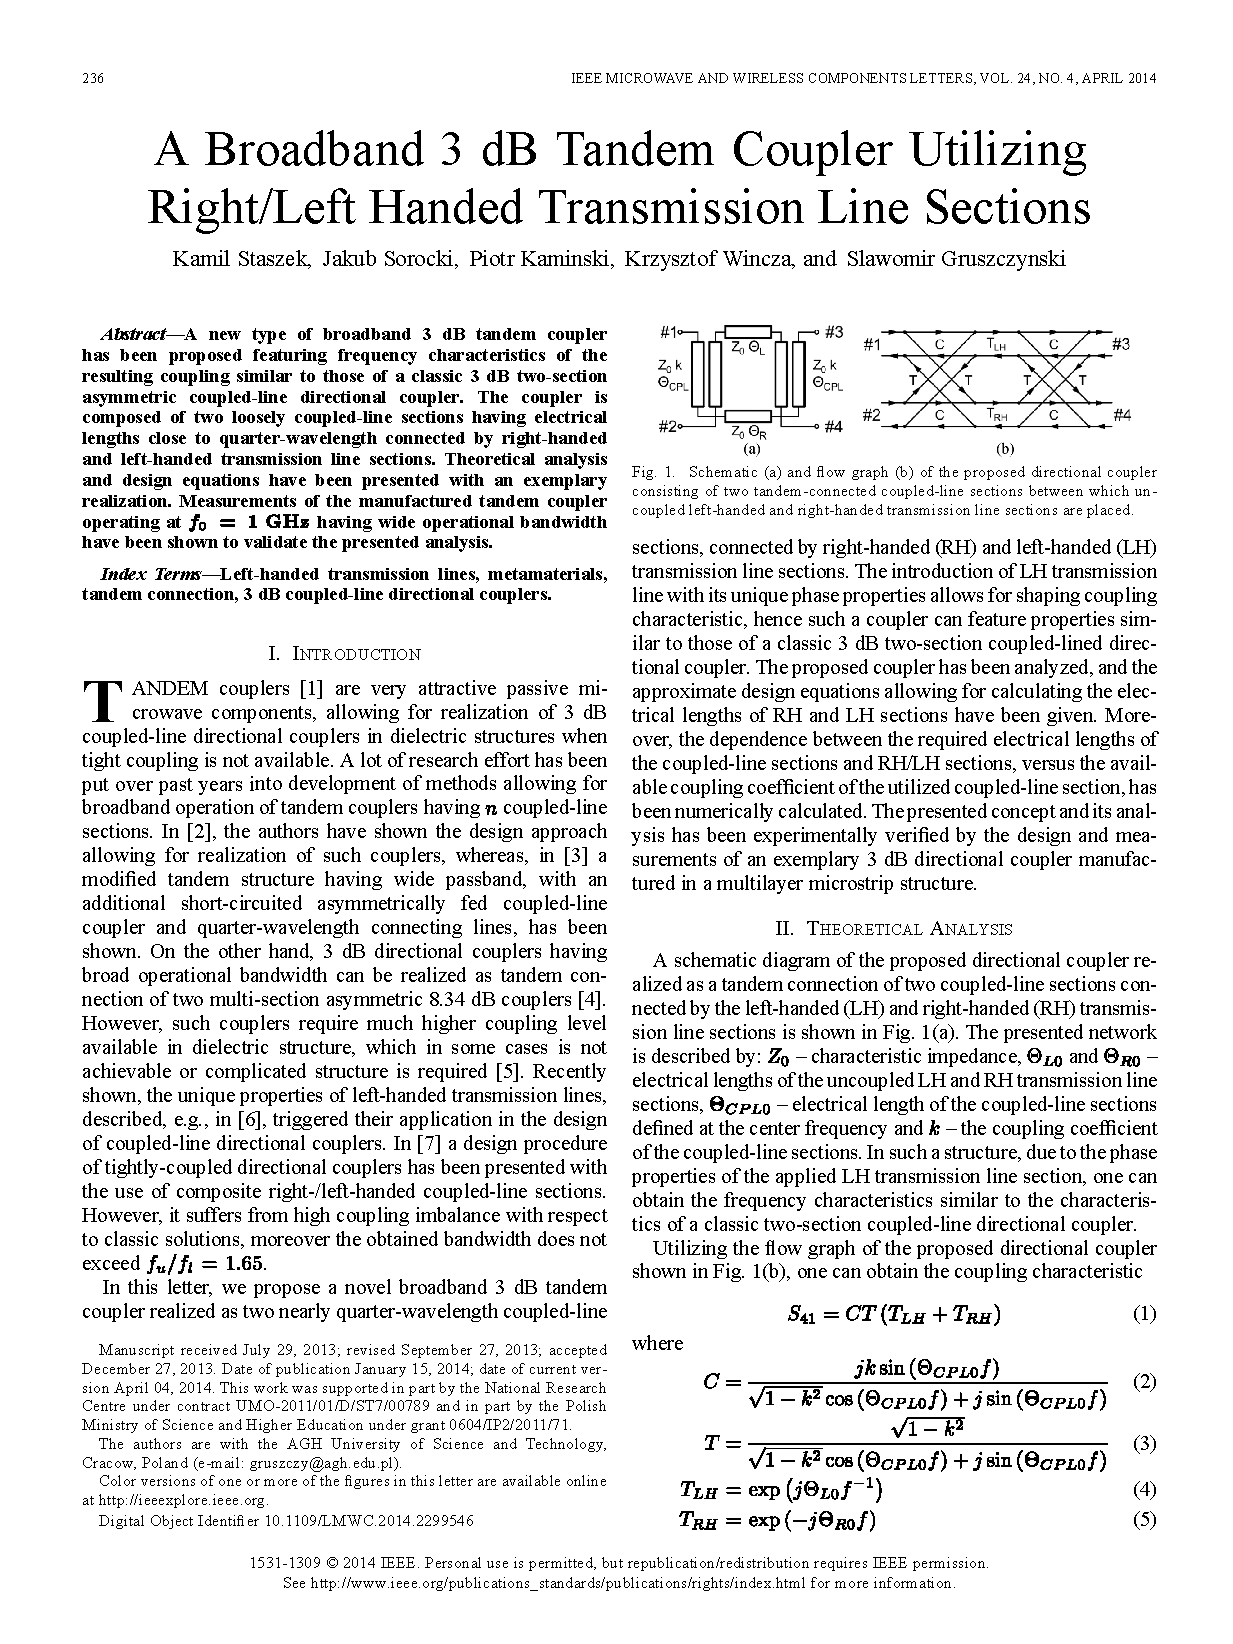
\includepdf[pages=-,addtotoc={1,section,1,A broadband 3 dB tandem coupler utilizing right/left handed transmission line sections,pe:mwcl_tandem}, pagecommand={}, scale=.97]{chapter_4/mwcl_tandem.pdf}

\cleardoublepage

%\includepdf[pages=-,addtotoc={1,section,1,Broadband balun circuits composed of impedance transforming directional couplers and LH transmission-line sections,tmtt_right_left}]{chapter_4/jiee.pdf}

%\cleardoublepage